 \documentclass[pdftex,12pt, oneside]{article}

%\usepackage[paperwidth=8.5in, paperheight=13in]{geometry} % Folio
\usepackage[paperwidth=8.27in, paperheight=11.69in]{geometry} % A4

\usepackage{makeidx}         % allows index generation
\usepackage{graphicx}        % standard LaTeX graphics tool
                             % when including figure files
\usepackage[bottom]{footmisc}% places footnotes at page bottom
\usepackage[english]{babel}
\usepackage{enumerate}
\usepackage{paralist}
\usepackage{float}
\usepackage{gensymb}  
\usepackage{listings}
\usepackage{color}
\usepackage{mathtools} % atau \usepackage{amsmath}
\renewcommand{\baselinestretch}{1.5}

\newcommand{\HRule}{\rule{\linewidth}{0.5mm}}

\definecolor{codegreen}{rgb}{0,0.6,0}
\definecolor{codegray}{rgb}{0.5,0.5,0.5}
\definecolor{codepurple}{rgb}{0.58,0,0.82}
\definecolor{backcolor}{rgb}{0.95,0.95,0.92}

\lstdefinestyle{mystyle}{
  backgroundcolor=\color{backcolor},
  commentstyle=\color{codegreen},
  keywordstyle=\color{magenta},
  stringstyle=\color{codepurple},
  basicstyle=\footnotesize,
  breakatwhitespace=false,
  breaklines=true,
  captionpos=b,
  keepspaces=true,
  numbers=left,
  numbersep=5pt,
  showspaces=false,
  showstringspaces=false,
  showtabs=false,
  tabsize=2
}

\lstset{style=mystyle}


\begin{document}
\sloppy % biar section ga melebar melewati kertas

\begin{center}
{\large RANCANGAN SISTEM BASIS DATA - WS PBB}
\\[1cm]
XX Februari 2017\\
Priyanto Tamami, S.Kom.
\end{center}

%\frontmatter%%%%%%%%%%%%%%%%%%%%%%%%%%%%%%%%%%%%%%%%%%%%%%%%%%%%%%


%%%%%%%%%%%%%%%%%%%%%%%%%%%%%%%%%%%%%%%%%%%%%%%%%%%%%%%%%%%%%%%%%%%%%%

\section{PENDAHULUAN}

Aplikasi \textit{Web Services} ini bertujuan untuk melakukan pencatatan pembayaran pada basis data SISMIOP yang dilakukan oleh Bank sebagai tempat pembayaran.

Aplikasi ini sesungguhnya tidak menggunakan basis data baru, melainkan menggunakan basis data yang sudah ada, yaitu basis data yang digunakan pada SISMIOP, dimana tabel yang terpengaruh atas pencatatan pembayaran ada dua, yaitu tabel SPPT, dan tabel PEMBAYARAN\_SPPT.

Agar setiap transaksi yang terjadi dapat dievaluasi penggunaannya, maka diperlukan tabel tambahan yang mencatat \textit{log} transaksi, baik pencatatan pembayaran, atau pembatalan pencatatan pembayaran (\textit{reversal}).


\section{STRUKTUR BASIS DATA}

Struktur basis data dapat digambarkan sebagai berikut :

\subsection{Struktur Tabel SPPT}

Tabel ini sebetulnya sudah terbentuk dan dimanfaatkan oleh aplikasi SISMIOP untuk menampung data tagihan Pajak Bumi dan Bangunan Perdesaan dan Perkotaan yang dihasilkan setiap tahun. Tabel ini akan digunakan dalam aplikasi \textit{Web Service} PBB sebagai data dasar penentuan jumlah pembayaran yang akan dikirimkan atas permintaan \textit{inquiry} dari Bank sebagai tempat pembayaran.

Strukturnya adalah seperti pada gambar \ref{fig:tabel-sppt} :

\begin{figure}[H]
  \centering
  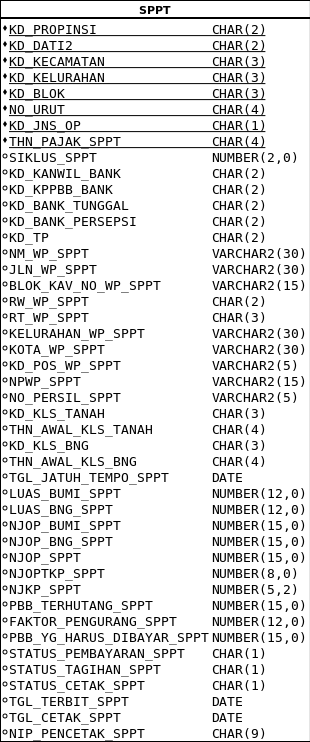
\includegraphics[width=0.4\textwidth]{./resources/01-struktur-tabel-sppt}
  \caption{Struktur Tabel SPPT}
  \label{fig:tabel-sppt}
\end{figure}

\subsection{Struktur Tabel PEMBAYARAN\_SPPT}

Tabel ini pun sudah terbentuk dan dimanfaatkan oleh aplikasi SISMIOP untuk mencatat transaksi pembayaran secara manual oleh operator. Tabel ini digunakan pula pada aplikasi \textit{Web Service} PBB untuk mencatat pembayaran yang terjadi.

Struktur dari tabel PEMBAYARAN\_SPPT ini adalah seperti pada gambar \ref{fig:tabel-pembayaran-sppt} :

\begin{figure}[H]
  \centering
  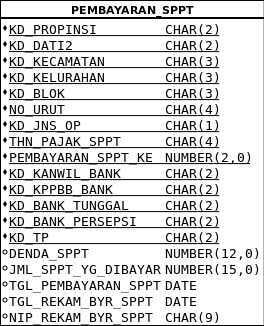
\includegraphics[width=0.4\textwidth]{./resources/02-struktur-tabel-pembayaran-sppt}
  \caption{Struktur Tabel PEMBAYARAN\_SPPT}
  \label{fig:tabel-pembayaran-sppt}
\end{figure}

\subsection{Struktur Tabel DAT\_OP\_BUMI}

Tabel ini sudah terbentuk dan dimanfaatkan oleh aplikasi SISMIOP untuk menampung data bumi dan objek pajak bumi dan bangunan. Tabel ini akan terisi pada saat operator memasukkan data-data pada lembar Surat Pemberitahuan Objek Pajak (SPOP). 

Struktur dari tabel DAT\_OP\_BUMI ini seperti pada gambar \ref{fig:tabel-dat-op-bumi} : 

\begin{figure}[H]
	\centering
	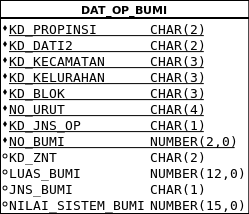
\includegraphics[width=0.4\textwidth]{./resources/03-struktur-tabel-dat-op-bumi}
	\caption{Struktur Tabel DAT\_OP\_BUMI}
	\label{fig:tabel-dat-op-bumi}
\end{figure}

\subsection{Struktur Tabel REF\_KELURAHAN}



\subsection{Struktur Tabel REF\_KECAMATAN}

\subsection{Struktur Tabel LOG\_TRX\_PEMBAYARAN}

\subsection{Struktur Tabel LOG\_REVERSAL}


\section{DIAGRAM RELASI \textit{ENTITY}}


\end{document}